

%(BEGIN_QUESTION)
% Copyright 2006, Tony R. Kuphaldt, released under the Creative Commons Attribution License (v 1.0)
% This means you may do almost anything with this work of mine, so long as you give me proper credit

De fleste frekvensomformere regulerer spenningen i forhold til frekvensen. Dette kalles V/f styring. Dette forholdet er ofte konstant for hele arbeidsområdet til motoren. 

For å forstå hvorfor spenningen må ha et fast forhold til frekvensen, kan det være til hjelp å bruke en spole til koblet en frekvensomformer. 


$$\includegraphics[width=15.5cm]{pk004x01.eps}$$


\underbar{file pk004.tex}
%\underbar{file i01441}
%(END_QUESTION)





%(BEGIN_ANSWER)

The inductor would most likely overheat and burn up.  As frequency decreases, so does inductive reactance ($X_L$).  As reactance decreases, there is less opposition in the inductor to AC current, so current increases proportionately.  This increased current will overheat the inductor (as well as saturate its magnetic core!).  Thus, we limit inductor current to its normal value through the inductor by reducing voltage as we reduce frequency.

%(END_ANSWER)





%(BEGIN_NOTES)


%INDEX% Final Control Elements, motor: variable-speed (volts/hertz ratio)

%(END_NOTES)


